
\begin{minipage}{0.58\linewidth}


La pyramide du Louvre à Paris est une pyramide régulière à base carrée de côté 35,42 m et de
hauteur 21,64 m. Elle est recouverte d’un vitrage composé de losanges et triangles de verre de
21,52 mm d’épaisseur. La densité du verre utilisé est de 2400 kg/m3.

\medskip

Estimer, en tonnes, le poids de la surface vitrée de ce monument.
\end{minipage}
\hfill
\begin{minipage}{0.38\linewidth}
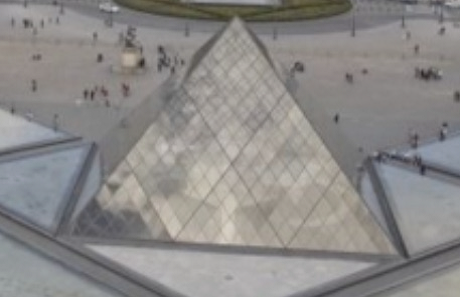
\includegraphics[scale=0.5]{RepS-pyramide_louvre.png} 
\end{minipage}
%%COMMENTAIRES: La résolution, qui nécessite le calcul de la hauteur et de l’aire d’un triangle, mobilise le
%théorème de Pythagore. L’enseignant, pour aider les élèves en difficulté, veille à ce que les
%représentations spatiales choisies conduisent à l’utilisation de cet outil.
%Une autre approche, plus ouverte, peut consister à fournir une photographie aérienne de la
%pyramide avec l’échelle, en laissant à la charge de l’élève le calcul de la longueur du côté de la
%base.
%Une autre piste est la construction d’une maquette à l’échelle ou, plus simplement, la
%construction d’une figure à l’aide d’un logiciel de géométrie dynamique. Dans ce dernier cas,
%l’enseignant peut éviter l’utilisation du théorème de Pythagore afin de calculer la hauteur d’un
%triangle isocèle (représentant chaque face de la pyramide). Il doit néanmoins, pour construire
%la figure et placer les sommets de la pyramide faire appel aux coordonnées cartésiennes
%(abscisse, ordonnée et altitude) de ces points.

